\section{Resultados e Discussões}
\label{sec:results}

Os experimentos desenvolvidos neste trabalho têm o intuito de verificar como variáveis socioeconômicas podem influenciar os tempos de acesso a pé aos pontos de interesse urbanos.

\subsection{Experimento 1 - Análise de Regressão}

O Experimento 1 resultou em um modelo de regressão linear com coeficiente de determinação (R²) de 0,73. Dentre as variáveis analisadas, 30 demonstraram efeitos estatisticamente significativos ($p < 0,005$). A Tabela \ref{tab:variaveis} (Apêndice A) detalha essas variáveis, incluindo seus nomes e descrições. A Figura \ref{fig:coef} apresenta os coeficientes e seus intervalos de confiança de 95\%, ordenados por magnitude de efeito. É importante destacar que as variáveis não foram padronizadas neste experimento. Portanto, embora a magnitude dos coeficientes não permita comparação direta sobre a influência relativa entre as variáveis, a direção do efeito (positiva ou negativa) mantém-se como um resultado relevante para a interpretação.

\begin{figure}[ht]
  \centering
  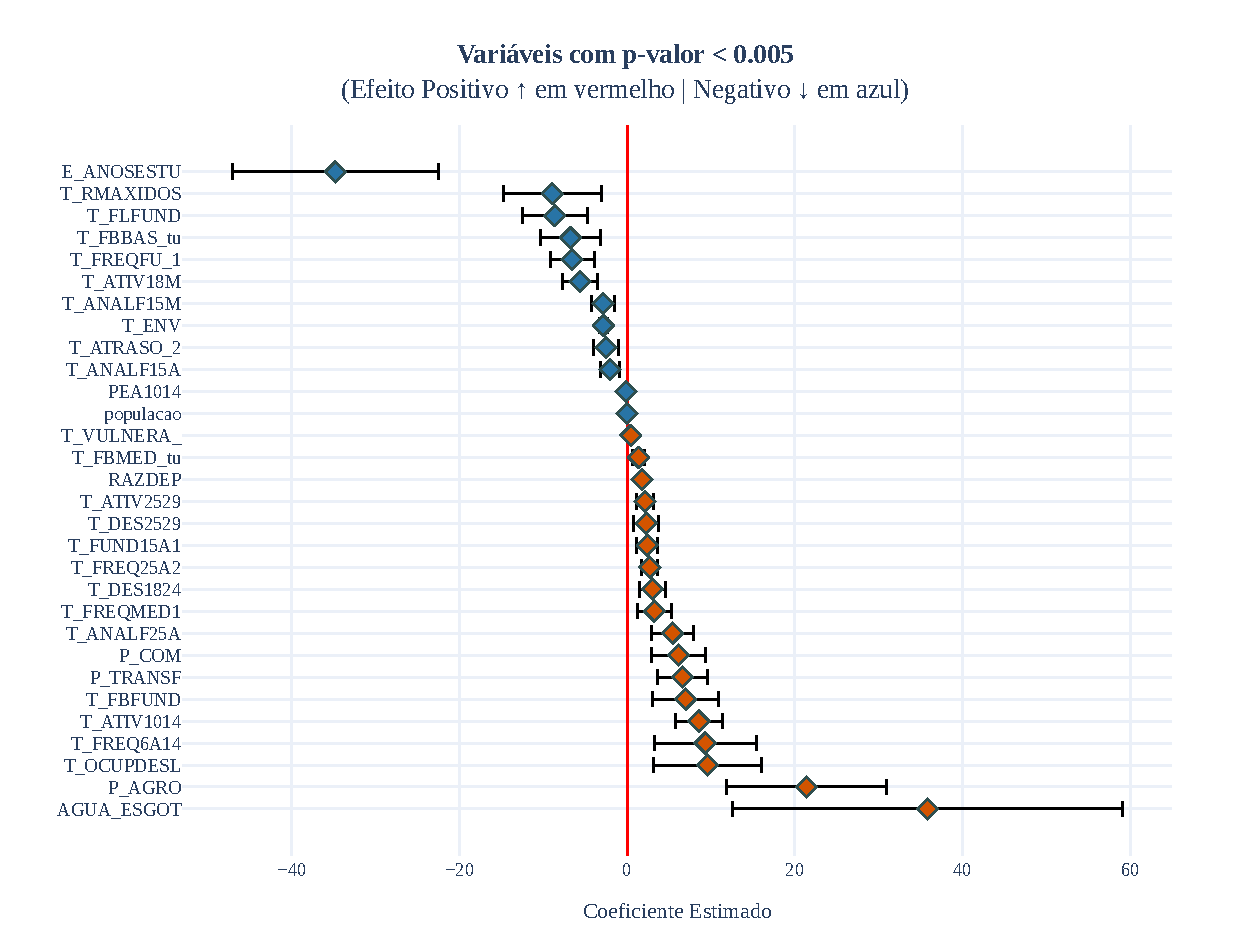
\includegraphics[width=0.8\textwidth]{figs/coeficientes.pdf} % Ou .svg/.eps
  \caption{Efeito das variáveis no tempo de acesso (IC95\%).}
  \label{fig:coef}
\end{figure}

O modelo identificou doze variáveis com associação negativa com o tempo de acesso, indicando que maiores valores nestes indicadores correspondem a menores tempos de deslocamento. Sete entre as doze variáveis com efeito negativo sugerem que áreas com melhores indicadores educacionais e maior participação econômica tendem a apresentar melhor acessibilidade urbana, sendo elas: (1) expectativa de anos de estudo aos 18 anos, (2) taxa de frequência líquida ao ensino fundamental, (3) taxa de frequência bruta ao ensino básico, (4) percentual da população de 15 a 17 anos frequentando o ensino fundamental, (5) taxa de pessoas maiores de 18 anos economicamente ativas, (6) taxa de envelhecimento e (7) tamanho da população.

O modelo também identificou cinco variáveis com indicadores sociais adversos que, paradoxalmente, apresentaram associação negativa com o tempo de acesso: (i) percentual de pessoas em domicílios vulneráveis à pobreza e dependentes de idosos, (ii) taxa de analfabetismo na população com mais de 15 anos, (iii) percentual de estudantes de 6 a 17 anos com atraso idade-série maior que 2 anos, (iv) taxa de analfabetismo na população de 15 a 17 anos, e (v) população economicamente ativa de 10 a 14 anos. Esses resultados aparentemente contraintuitivos podem sugerir tanto um artefato espacial (com a concentração dessas condições em áreas próximas a regiões centrais mais servidas por \ac{pois}) quanto a necessidade de investigar outros mecanismos subjacentes não capturados pelo modelo atual.

Dezoito variáveis apresentaram associação positiva com o tempo de acesso, sendo as mais intuitivas aquelas relacionadas a vulnerabilidades estruturais: (a) indicadores de inatividade juvenil, (b) razão de dependência demográfica (proporção de pessoas economicamente dependentes – crianças e idosos – em relação à população em idade ativa – entre 15 e 64 anos), (c) analfabetismo em adultos jovens (25-29 anos), e (d) concentração ocupacional em setores primários e comercio e taxa de desemprego de pessoas de 25 a 29 anos. Complementando esse perfil, destacam-se (e) trabalho infantil (atividade 10-14 anos) e (f) precariedade domiciliar (infraestrutura sanitária inadequada e longos tempos de deslocamento). Esses resultados confirmam expectativas teóricas sobre a penalidade de acessibilidade temporal em territórios com inserção econômica precária. 

Dentre essas dezoito variáveis, cinco apresentaram associações positivas que contrariam hipóteses iniciais: (g) taxa de frequência bruta ao ensino médio regular, (h) percentual de jovens de 18-24 anos no ensino médio regular, (i) taxa de frequência bruta ao ensino fundamental regular, (j) taxa de atendimento escolar (6-14 anos) e (k) taxa de atividade econômica (25-29 anos). Esses resultados inesperados destacam a complexidade da relação entre indicadores socioeconômicos e acessibilidade temporal urbana, revelando tanto limitações do modelo linear quanto mecanismos subjacentes não capturados pela análise. Esses resultados podem ser melhor compreendidos através da análise de clusterização desenvolvida no Experimento 2 que examina como a combinação dessas variáveis se distribui no território e compara as médias dos tempos de acesso entre os clusters identificados.

\subsection{Experimento 2 - Análise de Clusterização}

A clusterização foi realizada nas duas primeiras componentes principais (PC1 e PC2), que juntas explicam 63,2\% da variância total. Para interpretar os clusters, examinamos as cargas (loadings) das variáveis originais nas componentes PC1 e PC2, como mostra a Figura \ref{fig:loadings}. A primeira componente (PC1), responsável por 44,8\% da variância, está fortemente correlacionada com variáveis socioeconômicas, como renda e escolaridade, consolidando-se como um eixo de estratificação social. Já a segunda componente (PC2), que explica 18,4\% da variância, associa-se predominantemente ao tempo de acesso a \ac{pois} em diferentes categorias (variáveis A1 – A64), revelando um eixo de acessibilidade temporal.

\begin{figure}[ht]
  \centering
  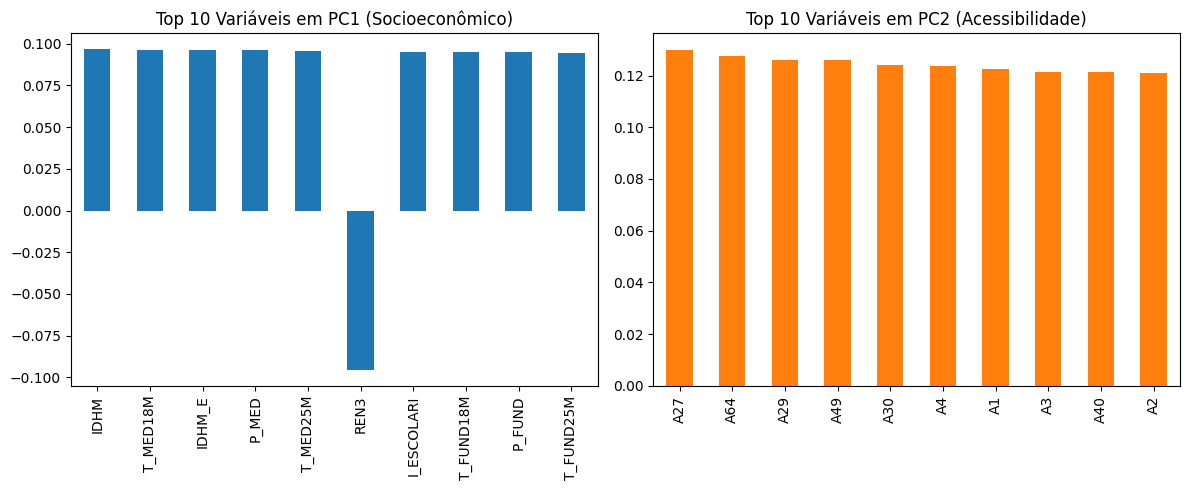
\includegraphics[width=\textwidth]{figs/top_pc_vars.png}
  \caption{Cargas das 10 variáveis mais influentes nas componentes principais PC1 e PC2.}
  \label{fig:loadings}
\end{figure}

O método do cotovelo indicou k=4 como um número adequado de clusters, cuja distribuição espacial é apresentada na Figura \ref{fig:clusters}. A análise revela quatro padrões territoriais distintos: o \textbf{Cluster 1 (Alto)} concentra-se em regiões centrais e bairros planejados, exibindo altas cargas positivas em PC1; o \textbf{Cluster 2 (Médio)} ocupa áreas adjacentes ao centro, com valores intermediários em ambas as componentes; o \textbf{Cluster 3 (Baixo)} caracteriza periferias consolidadas, marcadas por baixos valores em PC1 e PC2; enquanto o \textbf{Cluster 4 (Rural)} identifica periferias distantes de baixa densidade populacional, com cargas moderadamente baixas em PC1 e negativas em PC2, sugerindo vulnerabilidades socioespaciais moderadas e elevados tempos de acesso.

\begin{figure}[!htbp]
  \centering
  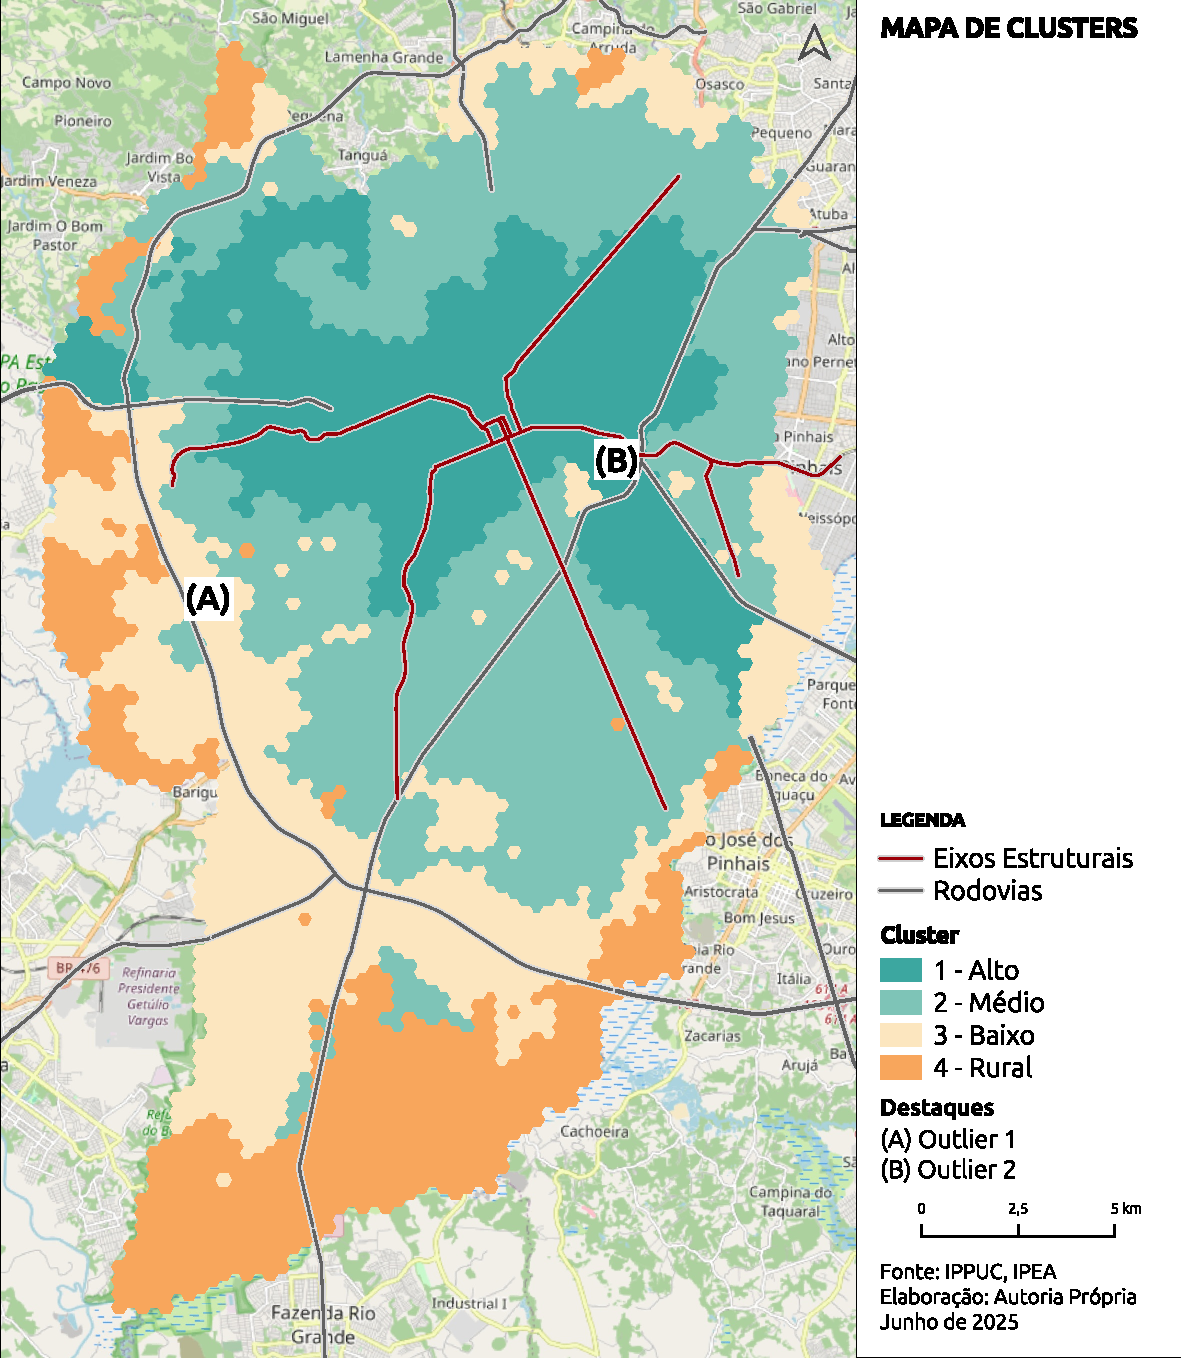
\includegraphics[width=0.6\textwidth]{figs/mapa_clusters_v2.pdf}
  \caption{Distribuição espacial dos clusters.}
  \label{fig:clusters}
\end{figure}

Os boxplots presentes na Figura \ref{fig:boxplots} revelam padrões claros de desigualdade entre os clusters. Para variáveis associadas a condições socioeconômicas favoráveis, como anos de estudo (E\_ANOSESTU) e frequência líquida ao ensino médio (T\_FLMED), observa-se uma gradativa redução das medianas e ampliação da dispersão à medida que se avança do Cluster 1 para o Cluster 3. O Cluster 1 apresenta distribuições concentradas em valores altos (ex.: mediana ao redor de 12,5 anos de estudo), enquanto o Cluster 3 exibe maior variabilidade e valores significativamente inferiores (ex.: mediana ao redor de 11,2 anos), refletindo disparidades educacionais. Já variáveis como T\_NESTUDA\_ (taxa de pessoas de 15 a 24 anos que não estudam e não trabalham e são vulneráveis a pobreza) e AGUA\_ESGOT (acesso inadequado a água e esgoto) seguem o padrão inverso, com piores indicadores no Clusters 3, corroborando a associação entre privação material e exclusão de serviços básicos.

A dimensão espacial também é evidente. O tempo de acesso a serviços (tempo\_acesso) é sistematicamente maior nos clusters periféricos (3 e 4), indicando que parte da população enfrenta deslocamentos excessivos. Em contraste, a expectativa de vida (ESPVIDA) tem queda abrupta para o Cluster 3 e o percentual de pessoas em domicílios com paredes que não sejam de alvenaria ou madeira aparelhada (PAREDE) tem aumento neste mesmo grupo, sugerindo que a combinação de baixos indicadores socioeconômicos e acessibilidade limitada potencializa vulnerabilidades.

A análise revela dois outliers: (A) uma vila residencial inserida em zona industrial, com uma densidade de \ac{pois} maior que a observado no Cluster 3, incluindo equipamentos públicos de qualidade, e indicadores de educação e infraestrutura superiores aos do entorno imediato; e (B) um assentamento precário em região central, cuja desorganização urbana (falta de pavimentação, ausência de equipamentos públicos) neutraliza completamente as vantagens da localização, aprofundando a exclusão socioespacial.

%\clearpage

\begin{figure}[!htbp]
{
  \centering
  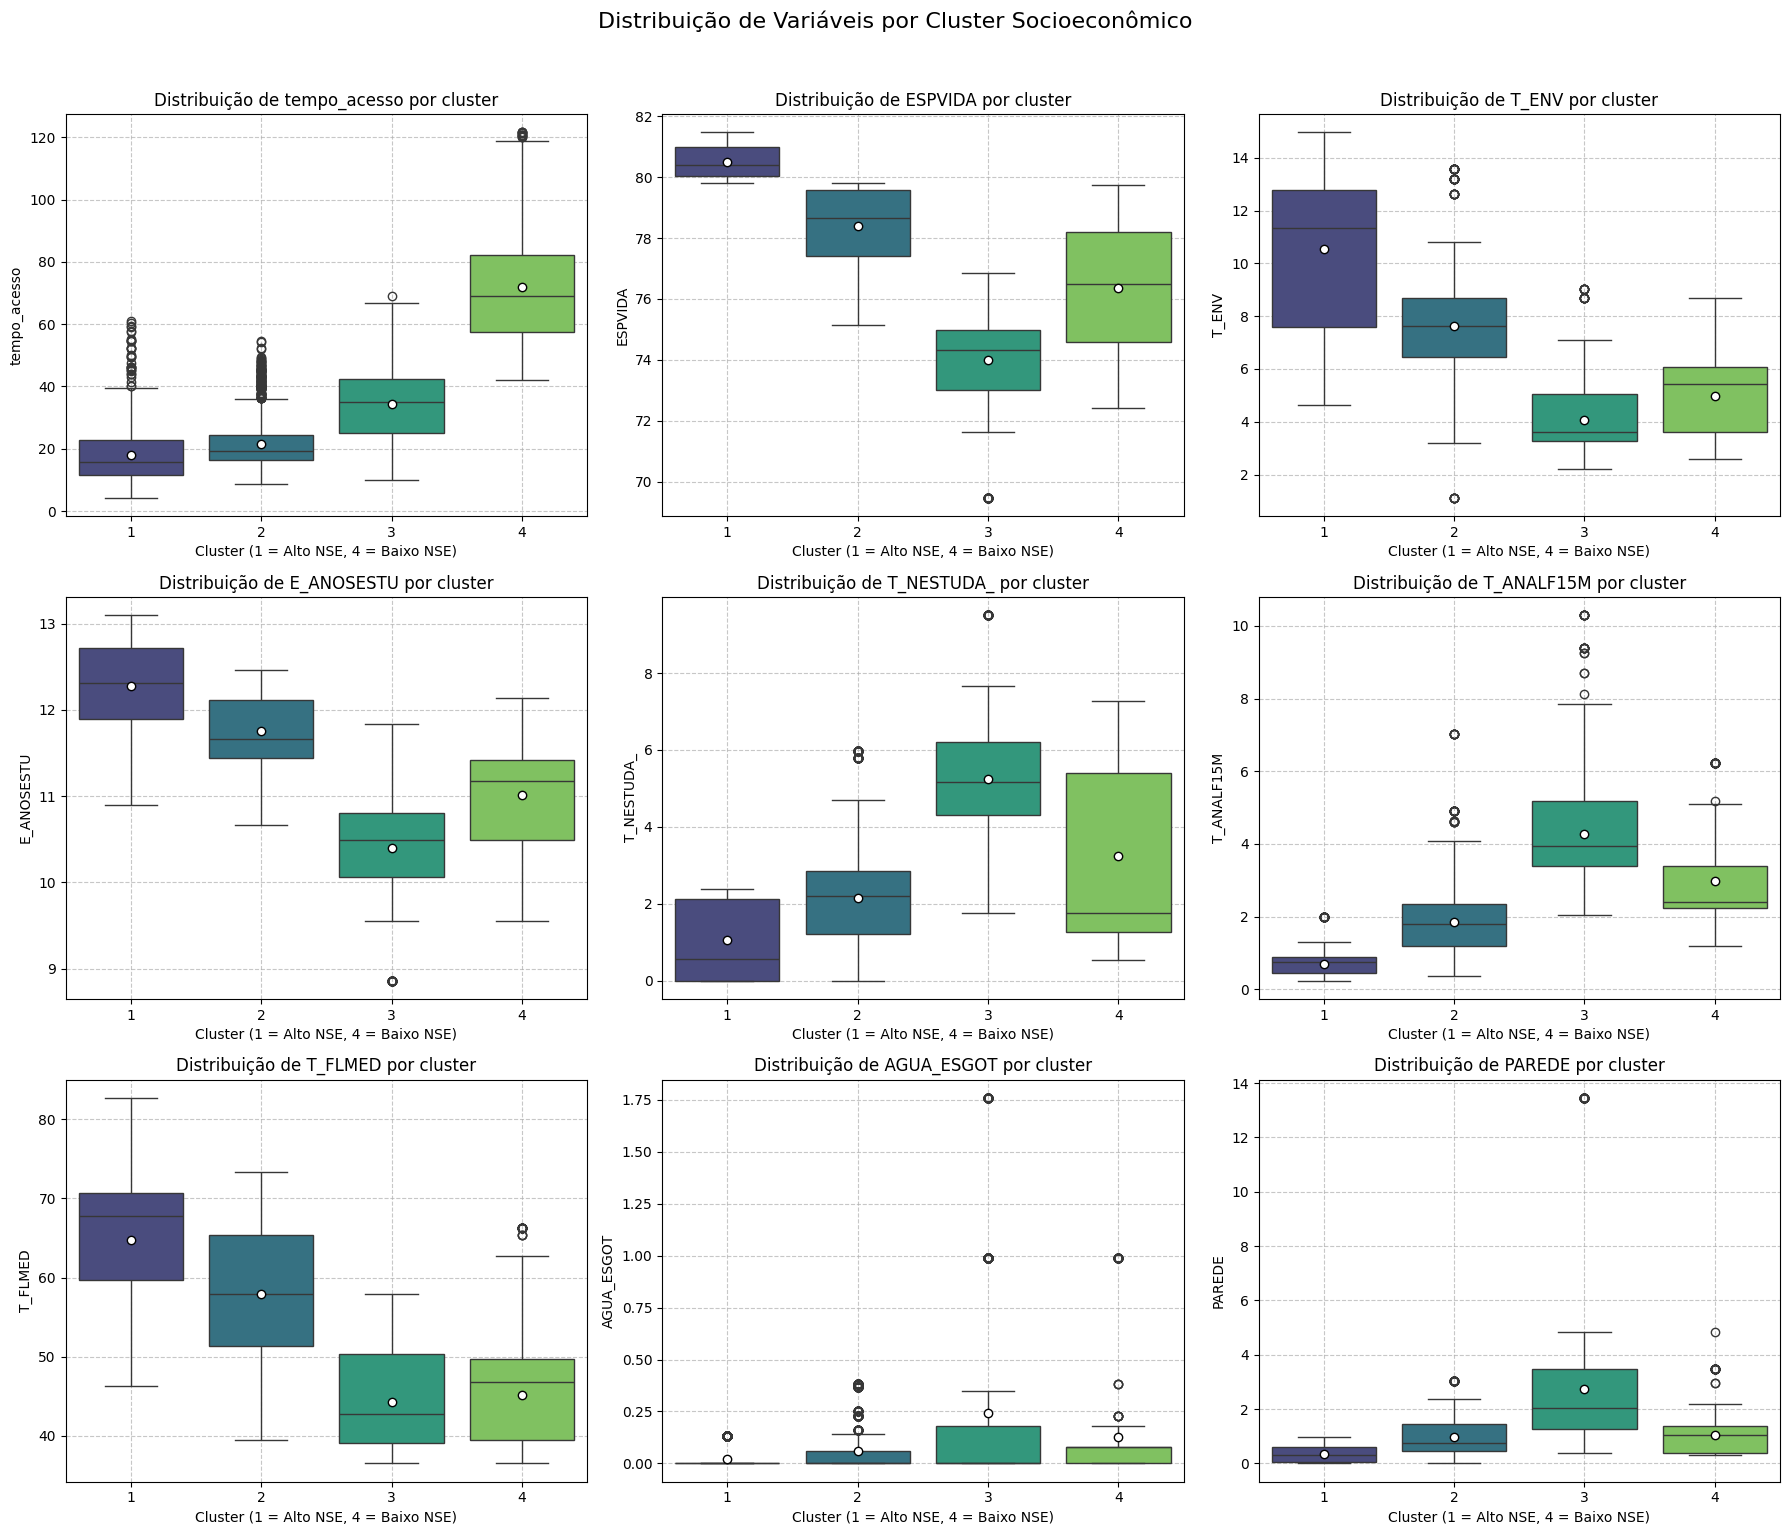
\includegraphics[width=\textwidth]{figs/cluster_boxplots.png}
  \caption{Distribuição de variáveis por cluster socioeconômico}
  \label{fig:boxplots}
}
\end{figure}